\documentclass[spanish]{llncs}   % llncs.cls esta en la ruta predefinida de TEX Live
\usepackage[colorlinks,citecolor=black,urlcolor=black,linkcolor=black,bookmarks=false,hypertexnames=true]{hyperref}
\usepackage{listingsutf8}
\usepackage{graphicx}
\usepackage[utf8]{inputenc}
\usepackage[section]{placeins}
\DeclareUnicodeCharacter{0301}{\'}

\begin{document}
\title{Práctica 9 - Obtención de Información Estructuradas y uso de Ontologías.}

\author{Hugo Pérez Fernández.  \email{UO250708@uniovi.es}
\institute{Sistemas de Información para la Web. Grado de Ingeniería Informática. EII. 
universidad de Oviedo. Campus de los Catalanes. Oviedo.}}
\maketitle              

\section{Introducción}

En esta práctica se verán las diferencias entre la obtención manual y automatica de la información estructurada para tres textos dados, 
ademas se trataran temas como por qué hay tantas ontologías y como tratar el problema de alinearlas a la hora de su uso. 

\section{Obtención manual de información estructurada}

Primero obtendremos toda la información estructurada de los textos indicados en el Anexo.\ref{Textos}, usando para ello la web \href{https://schema.org}{Schema.org}:

\paragraph{Texto 1:}

En el caso de este texto se esta mecionando a una persona (\textit{schema:Person}), cuyo nombre es Miles Davis, ademas esta persona tiene como nacionalidad \textit{schema:Nacionality}
Americano (Estadounidense), y su profesión (\textit{schema:Ocupation}) es músico concretamente de Jazz.

\paragraph{Texto 2:}

En en este caso la información se puede estructurar de la siguiente forma:

\begin{itemize}
    \item Hay y una persona (\textit{schema:Person}) que se llama Barack Obama cuya ocupación (\textit{schema:Ocupation}) es presidente.
    \item Hay una organizacion (\textit{schema:Organization}) que se llama Unión Europea.
    \item Hay una ciudad (\textit{schema:City}) que se llama Washington.
    \item Hay una tipo de cambio de moneda (\textit{schema:ExchangeRateSpecification}) que se llama Euro y tiene un valor de 1.3.
    \item Hay una reunion (\textit{schema:BusinessEvent}) entre Barack Obama y la Unión Europea
    sobre el el valor del tipo de cambio del Euro.
\end{itemize}

\paragraph{Texto 3:}

En este último se  puede estructura la información del siguiente modo:

\begin{itemize}
    \item Hay una organización (\textit{schema:Organization}) que se llama The New York Times.
    \item Hay una persona (\textit{schema:Person}) que se llama Jhon McCarthy.
    \item Jhon McCarthy está muerto.
    \item El New York Times informa (\textit{schema:Report}) que Jhon McCarthy esta muerto.
    \item LISP es un lenguaje de programación.
    \item John McCarthy inventó LISP.
\end{itemize}

Con los datos obtenidos anteriormente se, usando la notacion Turtle, la información estructurada queda de la siguiente manera:

\lstset{
    frame=tb, % draw a frame at the top and bottom of the code block
    tabsize=2, % tab space width
    showstringspaces=false, % don't mark spaces in strings
    numbers=left, % display line numbers on the left
    commentstyle=\color{green}, % comment color
    keywordstyle=\color{black}, % keyword color
    stringstyle=\color{blue}, % string color    
    inputencoding=utf8/latin1
}
\lstinputlisting[language=HTML, breaklines, caption={Archivo Turtle con la información estructurada de los textos.}]{resources/texts.ttl}

Ahora verificaremos la estructura de la sistaxis RDF de del archivo anterior mediante la herramienta \href{http://rdfshape.weso.es/dataInfo}{RDFShape}:

\begin{figure}[h]
    \centering
    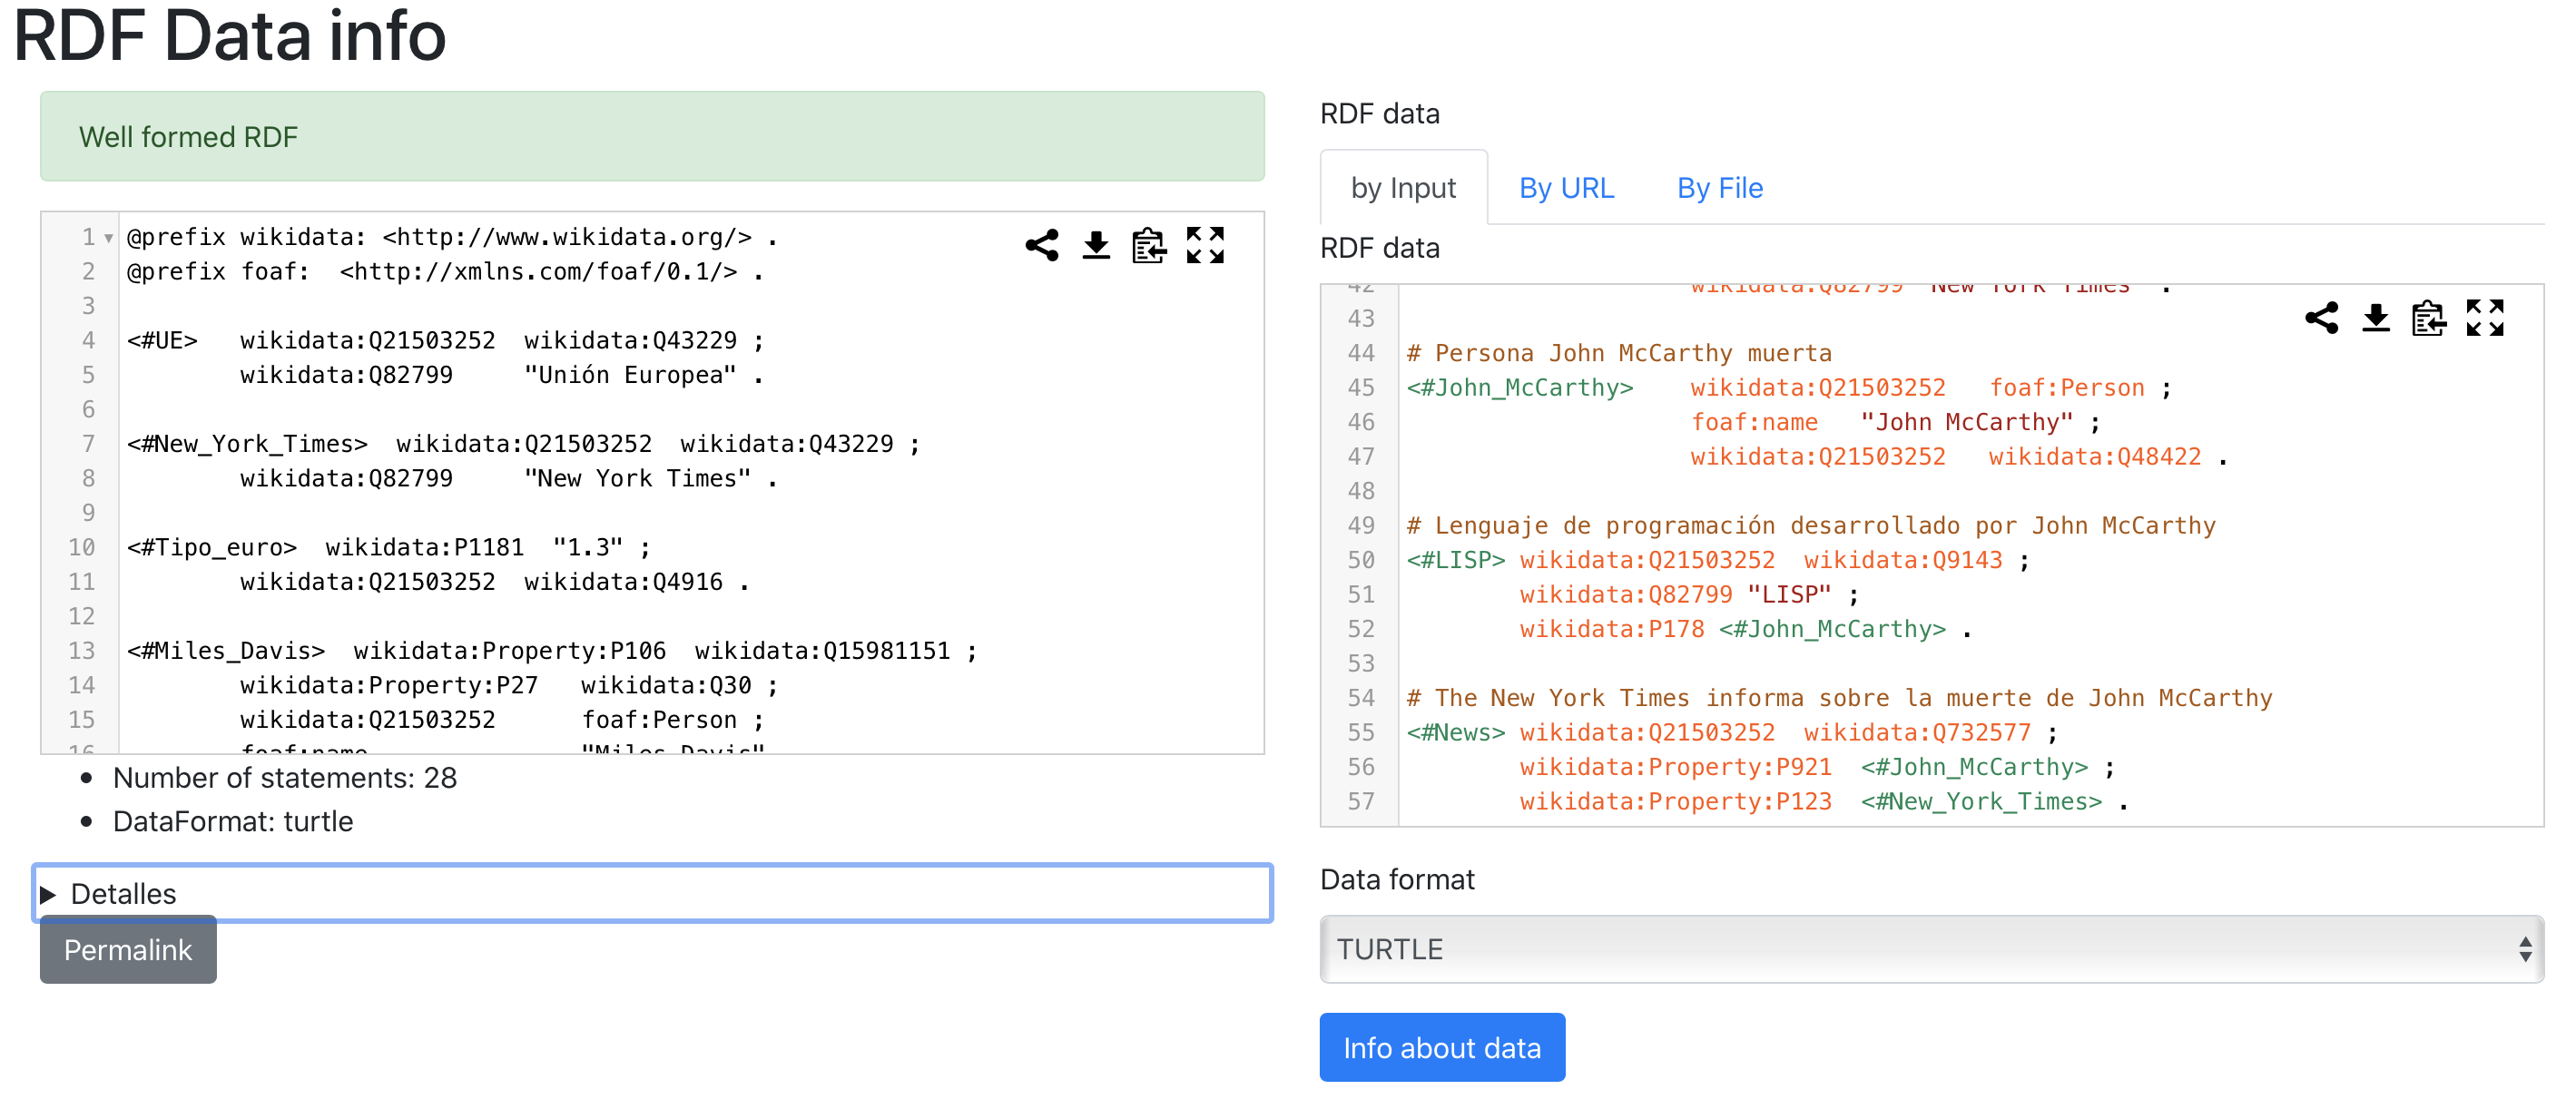
\includegraphics[width=\textwidth]{resources/RDFValidation.png}
    \caption{Resultado de la validación del ttl con RDFShape.}
    \label{Fig.1}
\end{figure}

Una vez verificado podemos traducir el formato turtle a JSONLD, usando para ello la herramienta \href{https://rdf-translator.appspot.com}{RDF-Translator}, de forma que quedaria de la siguiente manera:

\lstset{
    frame=tb, % draw a frame at the top and bottom of the code block
    tabsize=2, % tab space width
    showstringspaces=false, % don't mark spaces in strings
    numbers=left, % display line numbers on the left
    commentstyle=\color{green}, % comment color
    keywordstyle=\color{red}, % keyword color
    stringstyle=\color{black}, % string color    
    inputencoding=utf8/latin1
}
\lstinputlisting[language=HTML,breaklines,caption={Archivo Resultado de la traduccion de turtle a JSONLD.}, captionpos=b]{resources/jsonld.json}


\section{Obtención automática de información estructurada}

\subsection{Obtención de RDF's.}

En esta sección obtendremos los documentos RDF para cada texto, par ello usaremos las siguientes herramientas: 
\href{https://www.refinitiv.com/en/products/intelligent-tagging-text-analytics}{Open Calais} y 
\href{http://wit.istc.cnr.it/stlab-tools/fred/demo/?}{FRED}. En el caso de la herramienta recomendada en el guión de prácticas
\href{https://www.dbpedia-spotlight.org/demo/}{DBPedia-spotlight} no se hará uso de ella debido a que no exporta un archivo rdf de modo 
que la generación de este no sería automático como se indica en el titulo de la sección.

Los archivos resultantes se encuentran en el fichero comprimido adjunto en la tarea llamado \textit{informacionEstructuradaAutomatica.zip}, 
este fichero contendrá tanto los archivos RDF de cada texto como los  que posteriormente se habrán traduciodo a formato turtle y a JSONLD.

Dada esta información ahora podremos dar respuesta a las siguientes cuestiones:

\textbf{\textit{¿Qué ontologías usa cada servicio para "tipar" las instancias detectadas en el texto?}}

Las ontologías que usa cada servicio para \textit{"tipar"} las instacias son las siguientes:

\paragraph{Open Calais:} En el caso de esta herramienta para todos los textos usa las siguientes ontologías, estas son fáciles de obtener
de los archivos en formato turttle obtnidos de la traducción de los rdf.

\begin{itemize}
    \item http://s.opencalais.com/1/pred/
    \item http://www.w3.org/1999/02/22-rdf-syntax-ns
    \item http://www.w3.org/2000/01/rdf-schema
    \item http://www.w3.org/XML/1998/namespace
    \item http://www.w3.org/2001/XMLSchema
\end{itemize}

\paragraph{FRED:} En el caso de esta herramienta presenta diferencias en las ontologias usadas en funcion del texto puesto que 
en unos necesita mas que en otros. El conjunto de todas las ontologías usadas es el siguiente:

\begin{itemize}
    \item http://www.ontologydesignpatterns.org/ont/dul/DUL.owl
    \item http://www.essepuntato.it/2008/12/earmark
    \item http://www.ontologydesignpatterns.org/ont/fred/domain.owl
    \item http://www.ontologydesignpatterns.org/ont/vn/abox/role/
    \item http://www.ontologydesignpatterns.org/ont/cnlp/dependencies.owl
    \item http://ontologydesignpatterns.org/cp/owl/semiotics.owl
    \item http://www.ontologydesignpatterns.org/ont/fred/pos.owl
    \item http://www.ontologydesignpatterns.org/ont/boxer/boxer.owl
    \item http://www.ontologydesignpatterns.org/ont/boxer/boxer.owl
    \item http://www.ontologydesignpatterns.org/ont/fred/quantifiers.owl
    \item http://www.ontologydesignpatterns.org/ont/fred/quantifiers.owl
    \item http://www.w3.org/2002/07/owl
    \item http://www.w3.org/1999/02/22-rdf-syntax-ns
    \item http://www.w3.org/2000/01/rdf-schema
    \item http://schema.org/
    \item http://www.w3.org/XML/1998/namespace
    \item http://www.w3.org/2001/XMLSchema
\end{itemize}

\textbf{\textit{¿Existe algún tipo de dichas ontologías que pudiera considerarse equivalente a otro tipo en schema.org? 
Señala todos los casos que te hayas encontrado con cada servicio, indicando también (si fuera posible) qué propiedades 
de un tipo mapearían sobre propiedades del otro.}}

Existen muchos casos en los que un tipo de entidad de una de las ontologias usadas mapea con otro de Schema.org, algunos ejemplos son los siguientes:

En el caso de Open Calais nos encontramos con: 
\begin{itemize}
    \item La entidad "http://s.opencalais.com/1/type/em/e/Person" que en Schema.org sería "https://schema.org/Person", además en 
    este caso mapearían directamente los siguientes atributos: name.
    \item La entidad "http://s.opencalais.com/1/type/em/e/City" que en Schema.org sería "https://schema.org/City", además en este caso 
    mapearían directamente los siguientes atributos: name.
    \item La entidad "http://s.opencalais.com/1/type/em/e/Organization" que en Schema.org sería "https://schema.org/Organization", además 
    en este caso mapearían directamente los siguientes atributos: name y additionalType.
    \item La entidad "http://s.opencalais.com/1/type/tag/Industry" que en Schema.org sería "https://schema.org/industry".
    \item La entidad "http://s.opencalais.com/1/type/er/Company" que en Schema.org sería "https://schema.org/Corporation", además 
    en este caso mapearían directamente los siguientes atributos: name.
    \item La entidad "http://s.opencalais.com/1/type/em/r/Quotation" que en Schema.org sería "https://schema.org/Quotation", además en 
    este caso mapearían directamente los siguientes atributos: about, spokenByCharacter.
    \item La entidad "http://s.opencalais.com/1/type/em/e/PublishedMedium" que en Schema.ord sería "https://schema.org/Periodical", además en 
    este caso mapearían directamente los siguientes atributos: name.
    \item La entidad "http://s.opencalais.com/1/type/em/e/ProgrammingLanguage" que en Schema.ord sería https://schema.org/ComputerLanguage, además en 
    este caso mapearían directamente los siguientes atributos: name.   
\end{itemize}

Por otro lado en el caso de FRED nos encontramos con los siguientes casos:
\begin{itemize}
    \item La entidad http://www.w3.org/2002/07/owl/Class que en Schema.ord sería https://schema.org/Class, además en 
    este caso mapearían directamente los siguientes atributos: subObject.
    \item La entidad "http://www.ontologydesignpatterns.org/ont/fred/domain.owl/ProgrammingLanguage" que en Schema.ord sería https://schema.org/ComputerLanguage, además en 
    este caso mapearían directamente los siguientes atributos: name.
    \item La entidad "http://www.ontologydesignpatterns.org/ont/fred/domain.owl/Report" que en Schema.ord sería https://schema.org/Report.
\end{itemize}
Cabe destacar que en el caso de la herramienta FRED ya se usa Schema.org como ontología para la generación de los archivos.

\textbf{\textit{Reflexiona acerca de los motivos que pueden llevar a cada equipo de desarrolladores a producir una ontología propia. 
Investiga (someramente) sobre el problema de alineación de ontologías.}}

Puede haber diversas razones por las que un equipo de desarrolladores produzcan una ontología propia; la primera es que esta se cree por 
mero desconocimiento de la existencia previa que satisfaga sus necesidades, otra razon podría ser que quisieran que la ontologia fuera hecha 
a medida de sus necesidades, de modo que añadirían a cada entidad los atributos que deseasen para su proposito, ademas otra razón sería que 
si la creasen ellos podrían asegurar el mantenimiento de esta asegurando asi que no se descontinuase, como podria ocurrir con otras como wikiData 
o Schema.org, por ultimo cabría destacar la posibilidad de que sea un requerimiento del proyecto la creación de dicha ontología porque esta no exista 
o se necesita que sea cerrada.

En cuanto al problema de alineación entre ontologías esto se produce en el momento que la misma entidad está definidad en mas de una ontología y:
\begin{itemize}
    \item La nomenclatura de los atributos es distinta.
    \item En unas ontologías aparecen unos atributos y en otras no.
    \item La definicion es ligeramente distinta.
\end{itemize}
Esto produce que trabajar con varias de estas ontologías al mismo tiempo sea complejo y tedioso, por ejemplo en el caso de realizar consultas SPARQL, 
que mediante el uso de consultas federadas podriamos transformar las entidades de una ontología en las mismas de otra esto no se puede hacer directamente 
por lo anteriormente mencionado. Por ello en muchas ontologias se incluye en todas las entidades el atributo sameAs en el que se recoge una lista de equivalencias 
con otras ontologías, hay que mencionar que en el caso de wikiDatra esto se realiza de diferente manera de modo que las entidades en vez de tener un 
atributo sameAs con una lista de equivalencias poseen un atributo de equivalencia por cada ontología que tenga registrada para ello.

\textbf{\textit{Utiliza el servicio sameAs.org para localizar equivalencias para todos los tipos fundamentales de Open Calais, DBPedia 
Spotlight y FRED, así como los homólogos de Schema.org que detectaste. ¿Existe algún sevicio para el que no se disponga de información 
en sameAs.org?}}

El unico caso en el que he conseguido alguna equivalencia ha sido en el caso de la ontología de Schema.org, algunas de estas son las siguientes:

\lstset{
    frame=tb, % draw a frame at the top and bottom of the code block
    tabsize=2, % tab space width
    showstringspaces=false, % don't mark spaces in strings
    numbers=left, % display line numbers on the left
    commentstyle=\color{green}, % comment color
    keywordstyle=\color{red}, % keyword color
    stringstyle=\color{black}, % string color    
    inputencoding=utf8/latin1
}
\begin{lstlisting}[language=HTML, breaklines, caption={Equivalencias de sameAs.org para Schema.org.}, captionpos=b]
    [
  {
    "uri": "http://schema.org/Thing",
    "numDuplicates": "2",
    "duplicates": [
      "http://schema.org/Thing",
      "http://www.w3.org/2002/07/owl#Thing"
    ]
  },
  {
    "uri": "http://purl.org/vocabularies/princeton/wn30/synset-person-noun-1",
    "numDuplicates": "12",
    "duplicates": [
      "http://dbpedia.org/ontology/Person",
      "http://dbpedia.org/ontology/PokerPlayer",
      "http://proton.semanticweb.org/protonu#Profession",
      "http://purl.org/vocabularies/princeton/wn30/synset-person-noun-1",
      "http://schema.org/Person",
      "http://sw.opencyc.org/2009/04/07/concept/en/_http___dbpedia_org_ontology_PokerPlayer_",
      "http://umbel.org/umbel#PersonTypes",
      "http://umbel.org/umbel/rc/PersonWithOccupation",
      "http://www.w3.org/2000/10/swap/pim/contact#Person",
      "http://xmlns.com/foaf/0.1/Person"
    ]
  },
  {
    "uri": "http://schema.org/Organization",
    "numDuplicates": "8",
    "duplicates": [
      "http://dbpedia.org/ontology/Organisation",
      "http://proton.semanticweb.org/protont#Organization",
      "http://proton.semanticweb.org/protonu#SportOrganization",
      "http://purl.org/vocabularies/princeton/wn30/synset-organization-noun-1",
      "http://schema.org/Organization",
      "http://umbel.org/umbel/rc/Organization",
      "http://umbel.org/umbel/rc/Organizations",
      "http://xmlns.com/foaf/0.1/Organization"
    ]
  },
  {
    "uri": "http://schema.org/City",
    "numDuplicates": "507",
    "duplicates": [
      "http://dbpedia.org/ontology/City",
      "http://dbpedia.org/resource/City",
      "http://dbpedia.org/resource/Town",
      "http://dbpedia.org/resource/Citie",
      "http://dbpedia.org/resource/Shahr",
      "http://dbpedia.org/resource/Cities",
      "http://dbpedia.org/resource/Cittie",
      "http://dbpedia.org/resource/CittA ",
      "http://dbpedia.org/resource/Ciudad",
      "http://dbpedia.org/resource/Citties",
      "http://dbpedia.org/resource/Pilseta",
      "http://dbpedia.org/resource/City_work",
      "http://dbpedia.org/resource/Porkberry"
    ]
  }
]
\end{lstlisting}

Al realizar este apartado no he conseguido para el resto de ontologìas que la web sameAs.org funcione, he probado con los tipos 
básicos de cada ontología asegurandome que tuviese un atributo sameAs pero aun asi no funciona como se observa en la siguientes imagenes.

\begin{figure}[!htb]
    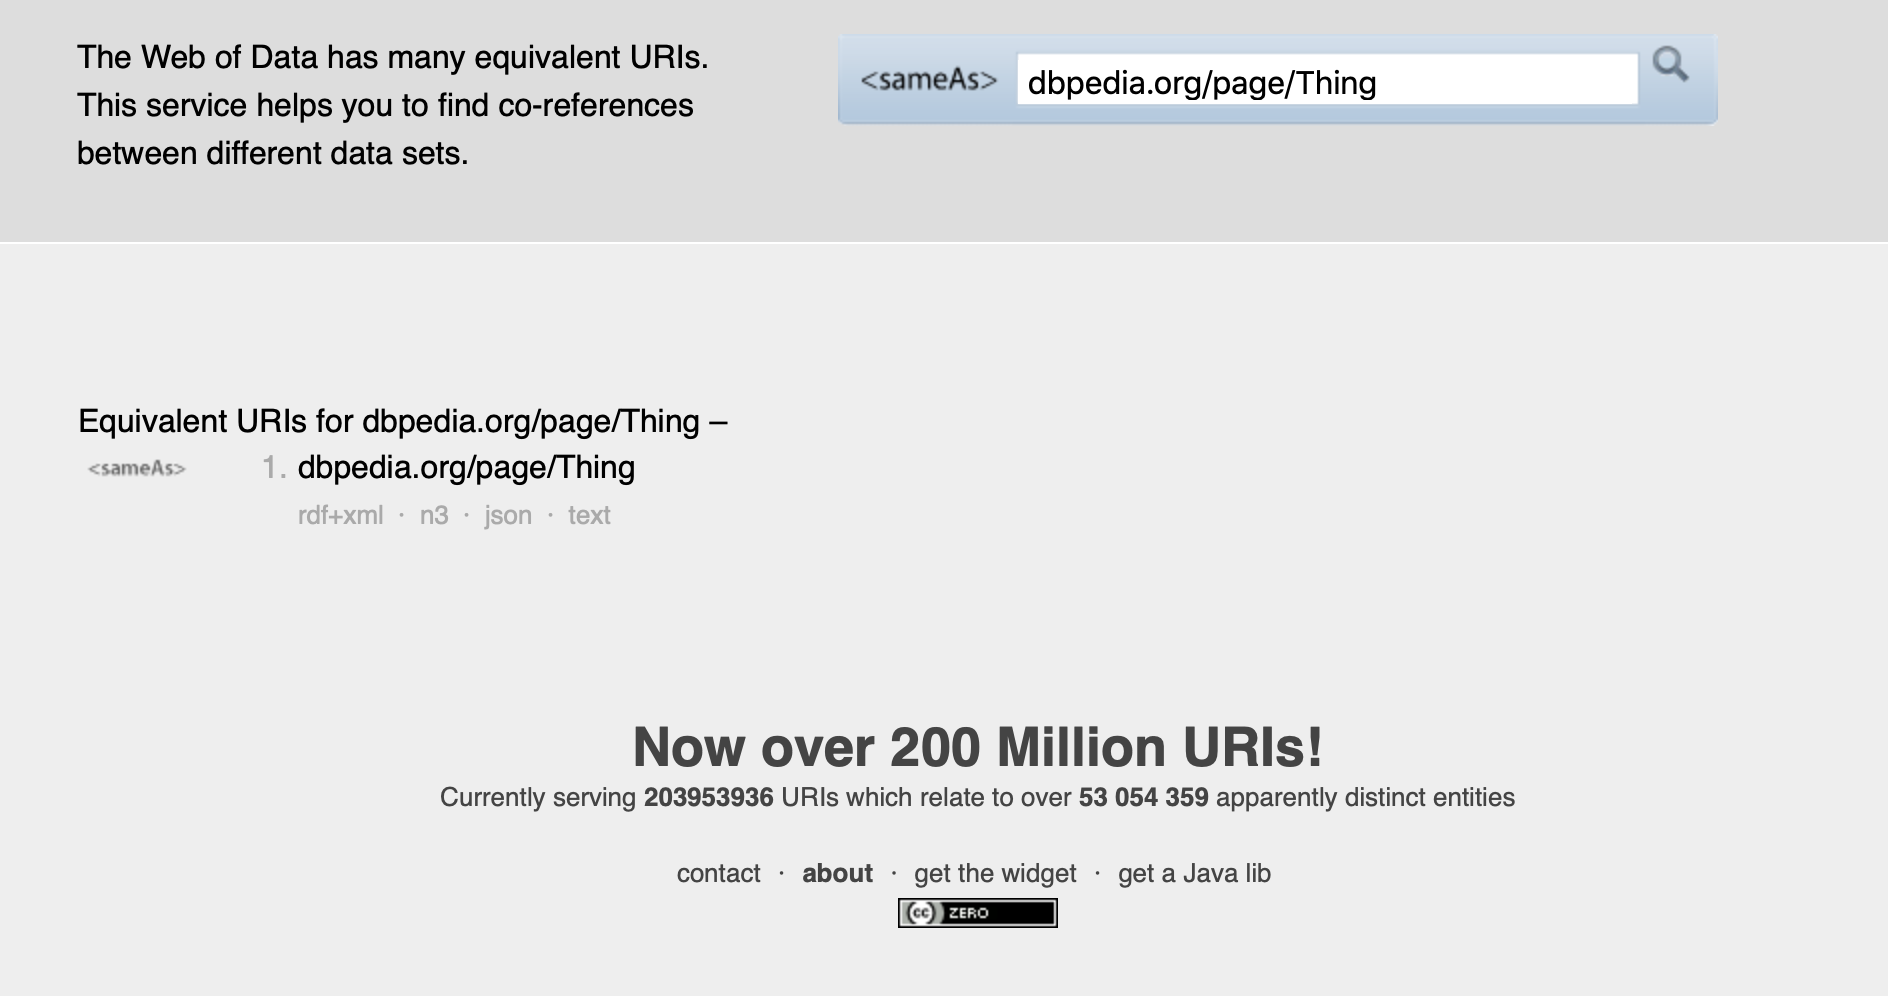
\includegraphics[width=\textwidth]{resources/SameAsWeb.png}
    \caption{Resultado la busqueda de http://dbpedia.org/page/Thing en SameAs.org.}
    \label{Fig.2}
    
\includegraphics[width=\textwidth]{resources/DBPediaSameAs.png}
    \caption{Resultado acceder de http://dbpedia.org/page/Thing y buscar el atributo sameAs.}
    \label{Fig.3}
\end{figure}

\section{Anexos}

\subsection{Textos de Prueba}\label{Textos}

\paragraph{Texto 1:}
“Miles Davis was an american jazz musician.”

\paragraph{Texto 2:}
“President Barack Obama and European Union leaders huddled in Washington amid growing fears over the future of the euro, which closed greater than 1.3 dollars.”

\paragraph{Texto 3:}
“The New York Times reported that John McCarthy died. He invented the programming language LISP.”

\end{document}